%%%%%%%%%%%%%%%%%%%%%%%%%%%%%%%%%%%%%%%%%%%%%%%%%%%%%%%%%%%%%%%%%%%%%%%%%%%%
%                                                                          %
% This is the LaTeX source of a Project Gutenberg eBook, online at         %
% https://www.gutenberg.org. Please find the license for this eBook at     %
% https://www.gutenberg.org/license                                        %
%                                                                          %
%%%%%%%%%%%%%%%%%%%%%%%%%%%%%%%%%%%%%%%%%%%%%%%%%%%%%%%%%%%%%%%%%%%%%%%%%%%%
%%
%% Producer’s Comments:
%%
%% The packages below are required for the purposes noted
%%
%% Summary of log file:
%% * No overfull vboxes
%% * No overfull hboxes
%% * No underfull hboxes
%% * No underfull vboxes
%%
%% Compile sequence:
%% latexmk -lualatex <filename>
%%

\listfiles
\documentclass[12pt,oneside]{book}[2021/10/04]

\usepackage{unicode-math}[2020/01/31]
\usepackage{yfonts}[2019/04/04] %for gothic
\usepackage{mathtools}[2021/02/02] %% for multlined and shortintertext

% STIX Two seems to have a problem with tables giving overfull hboxes
% so use something else
\setmainfont{XITS}
\setmathfont{XITS Math}

\setlength{\paperwidth}{14.87cm}%
\setlength{\paperheight}{21.02cm}%

\usepackage[
  top=0.8cm,
  bottom=0.5cm,
  left=0.81cm,
  right=0.81cm,
  headheight=17pt, % as per the warning by fancyhdr
  includehead,includefoot,
  heightrounded, % to avoid spurious underfull messages
]{geometry}[2020/01/02]% Page Geometry

\usepackage{letterspace}[2021/12/10] % letterspacing
\usepackage{setspace}[2011/12/19] % line spacing

\usepackage{dcolumn}[2014/10/28] % for tables with aligned numbers
\usepackage{enumitem}[2019/06/20] % Customized lists
\usepackage[perpage, para]{footmisc}[2011/06/06] % for footnotes anchors
\usepackage{multirow}[2021/03/15] % for tables with a cell spanning 2+ rows in other columns
\usepackage{bigstrut}[2021/03/15] % for multirow entries in table
\usepackage{rotating}[2016/08/11] % for sidewaystable
\usepackage{caption}[2020/01/03] % for table captions
\usepackage{float}[2001/11/08] % for H option with table
\usepackage{bigdelim}[2019/05/31] % for bracketed table rows
\usepackage{footnote}[1997/01/28]
\usepackage{titlesec}[2019/10/16] % for section styling
% need parskip. It doesn't have effect here because skip=0 but it prevents
% interaction with titles when skip is changed in pg boilerplate
\usepackage[skip=0pt plus1pt, indent=1.5em]{parskip}[2021-03-14] % parskip adjustments
\usepackage{fancyhdr}[2019/01/31] % for page headers
\usepackage{indentfirst}[1995/11/23] % indent first paragraph in sections
\usepackage{flafter}[2021/07/31] % force floats to appear after declaration, not before
\usepackage[
  pdfpagelayout=SinglePage,
  pdfdisplaydoctitle,
  colorlinks=true,
  linkcolor=blue,
]{hyperref}[2021-06-07] % Hypertext links for LaTeX

% [math-style=french] gives upright capital letters
% but also upright lower case greek so do this instead
% make upright capital letters
\DeclareSymbolFont{upletters}{T1}{cmr}{m}{n}
\SetSymbolFont{upletters} {bold}{T1}{cmr} {b}{n}
\DeclareSymbolFontAlphabet{\mathnormal}{upletters}
\DeclareMathSymbol{A}{\mathalpha}{upletters}{`A}
\DeclareMathSymbol{B}{\mathalpha}{upletters}{`B}
\DeclareMathSymbol{C}{\mathalpha}{upletters}{`C}
\DeclareMathSymbol{D}{\mathalpha}{upletters}{`D}
\DeclareMathSymbol{E}{\mathalpha}{upletters}{`E}
\DeclareMathSymbol{F}{\mathalpha}{upletters}{`F}
\DeclareMathSymbol{G}{\mathalpha}{upletters}{`G}
\DeclareMathSymbol{H}{\mathalpha}{upletters}{`H}
\DeclareMathSymbol{I}{\mathalpha}{upletters}{`I}
\DeclareMathSymbol{J}{\mathalpha}{upletters}{`J}
\DeclareMathSymbol{K}{\mathalpha}{upletters}{`K}
\DeclareMathSymbol{L}{\mathalpha}{upletters}{`L}
\DeclareMathSymbol{M}{\mathalpha}{upletters}{`M}
\DeclareMathSymbol{N}{\mathalpha}{upletters}{`N}
\DeclareMathSymbol{O}{\mathalpha}{upletters}{`O}
\DeclareMathSymbol{P}{\mathalpha}{upletters}{`P}
\DeclareMathSymbol{Q}{\mathalpha}{upletters}{`Q}
\DeclareMathSymbol{R}{\mathalpha}{upletters}{`R}
\DeclareMathSymbol{S}{\mathalpha}{upletters}{`S}
\DeclareMathSymbol{T}{\mathalpha}{upletters}{`T}
\DeclareMathSymbol{U}{\mathalpha}{upletters}{`U}
\DeclareMathSymbol{V}{\mathalpha}{upletters}{`V}
\DeclareMathSymbol{W}{\mathalpha}{upletters}{`W}
\DeclareMathSymbol{X}{\mathalpha}{upletters}{`X}
\DeclareMathSymbol{Y}{\mathalpha}{upletters}{`Y}
\DeclareMathSymbol{Z}{\mathalpha}{upletters}{`Z}

% redefine as mathord instead of mathbin
\DeclareMathSymbol{·}{\mathord}{symbols}{"00B7}

\titleformat*{\section}{\sc \center}

\newcommand{\ie}{\textit{i.e.}}
\newcommand{\bigsurd}{\sqrt{\vphantom{\frac{A}{B}}}}
\newenvironment{letlist}{\begin{description}[leftmargin=4em, itemindent=-2em]}{\end{description}}

\newenvironment{tnote}{
  \clearpage
  \setlength\parskip{5pt plus1pt}
  \raggedright
}
{
}

\newcommand{\ldot}{\,.\,}
\newcommand{\bdots}{\multicolumn{1}{c|}{\dots}}
% dots with extra separator line
\newcommand{\edots}{\multicolumn{1}{c||}{\dots}}
\newcommand{\hangind}[1]{\noindent \hangindent=2em {#1}\par}
\newcommand{\strutb}{\rule[-8pt]{0pt}{26pt}}
\newcommand{\sstrut}{\rule[0pt]{0pt}{18pt}}
\newcommand{\estrut}{\rule[-10pt]{0pt}{18pt}}
\newcommand{\xp}{\rule[-2.2ex]{0pt}{3.4ex}}
\newcommand{\xpa}{\rule[-1.6ex]{0pt}{3.4ex}}

% this is used instead of a math markup when there is a footnote in the centred text.
\newenvironment{tightcenter}{%
  \setlength\topsep{2pt}
  \setlength\parskip{2pt}
  \begin{center}
}{%
  \end{center}
}

\newcolumntype{d}{D{.}{·}{-1}}
\newcolumntype{e}{D{.}{·}{0.6}}
\newcolumntype{g}{D{.}{·}{4.1}}
\newcolumntype{h}{D{.}{·}{1.3}}
\newcolumntype{j}[1]{D{.}{·}{#1}}

\renewcommand{\thefootnote}{\fnsymbol{footnote}}
\newcommand{\fspace}{1.2cm}
\newcommand{\doubleline}{\moveright 0.25\textwidth \vbox{\hrule width 0.5\textwidth \kern 1mm \hrule width 0.5\textwidth}}
\newcommand{\singleline}{\moveright 0.25\textwidth \vbox{\hrule width 0.5\textwidth}}
\renewcommand{\headrulewidth}{0pt}
\newcommand{\coldash}{\multicolumn{1}{c}{—}}

\newfontfamily\blockfont{DejaVu Sans}[Scale=MatchUppercase]

% avoid overfull hboxes
\emergencystretch 2em%


\usepackage{fontspec}[2022/01/15] % for font selection
\usepackage{array}[2021/10/04] % for >{\raggedright\arraybackslash} in tabular
\usepackage{fancyhdr}[2019/01/31] % for page headers
\usepackage{graphicx}[2021/09/16] % for images and scalebox
\usepackage{hyperref}[2021-06-07] % Hypertext links for LaTeX

\graphicspath{ {./images/} }

% for PG text use a sans font similar size to stix2, some others are much bigger
\newfontfamily\pgfont{Alegreya Sans}
\newenvironment{PGtext}{\thispagestyle{empty}
\raggedright \pgfont
\setlength\parskip{5pt plus1pt}}{}

\newcommand{\PGLicense}{%
  \clearpage
  \pagestyle{fancy}
  \fancyhf{}
  \pagenumbering{Roman}
  \fancyhead[L]{}
  \fancyhead[C]{\small \pgfont License}
  \fancyhead[R]{\thepage}
  \renewcommand{\headrulewidth}{0pt}
}

\newcommand{\LicenseSection}[1]{\subsection*{\pgfont\normalsize\bfseries #1}}

\begin{document}
\hypersetup{
    pdftitle={On the relation which ought to subsist between the strength of an electric current and the diameter of conductors, to prevent overheating},
    pdfauthor={George Forbes},
    pageanchor=false,
    pdfdisplaydoctitle=true,
    colorlinks=true,
    urlcolor=blue,
}

\newgeometry{ % let image fill page
  top=0cm,
  bottom=0cm,
  left=0cm,
  right=0cm,
}
\thispagestyle{empty}
\begin{figure}[tbp]
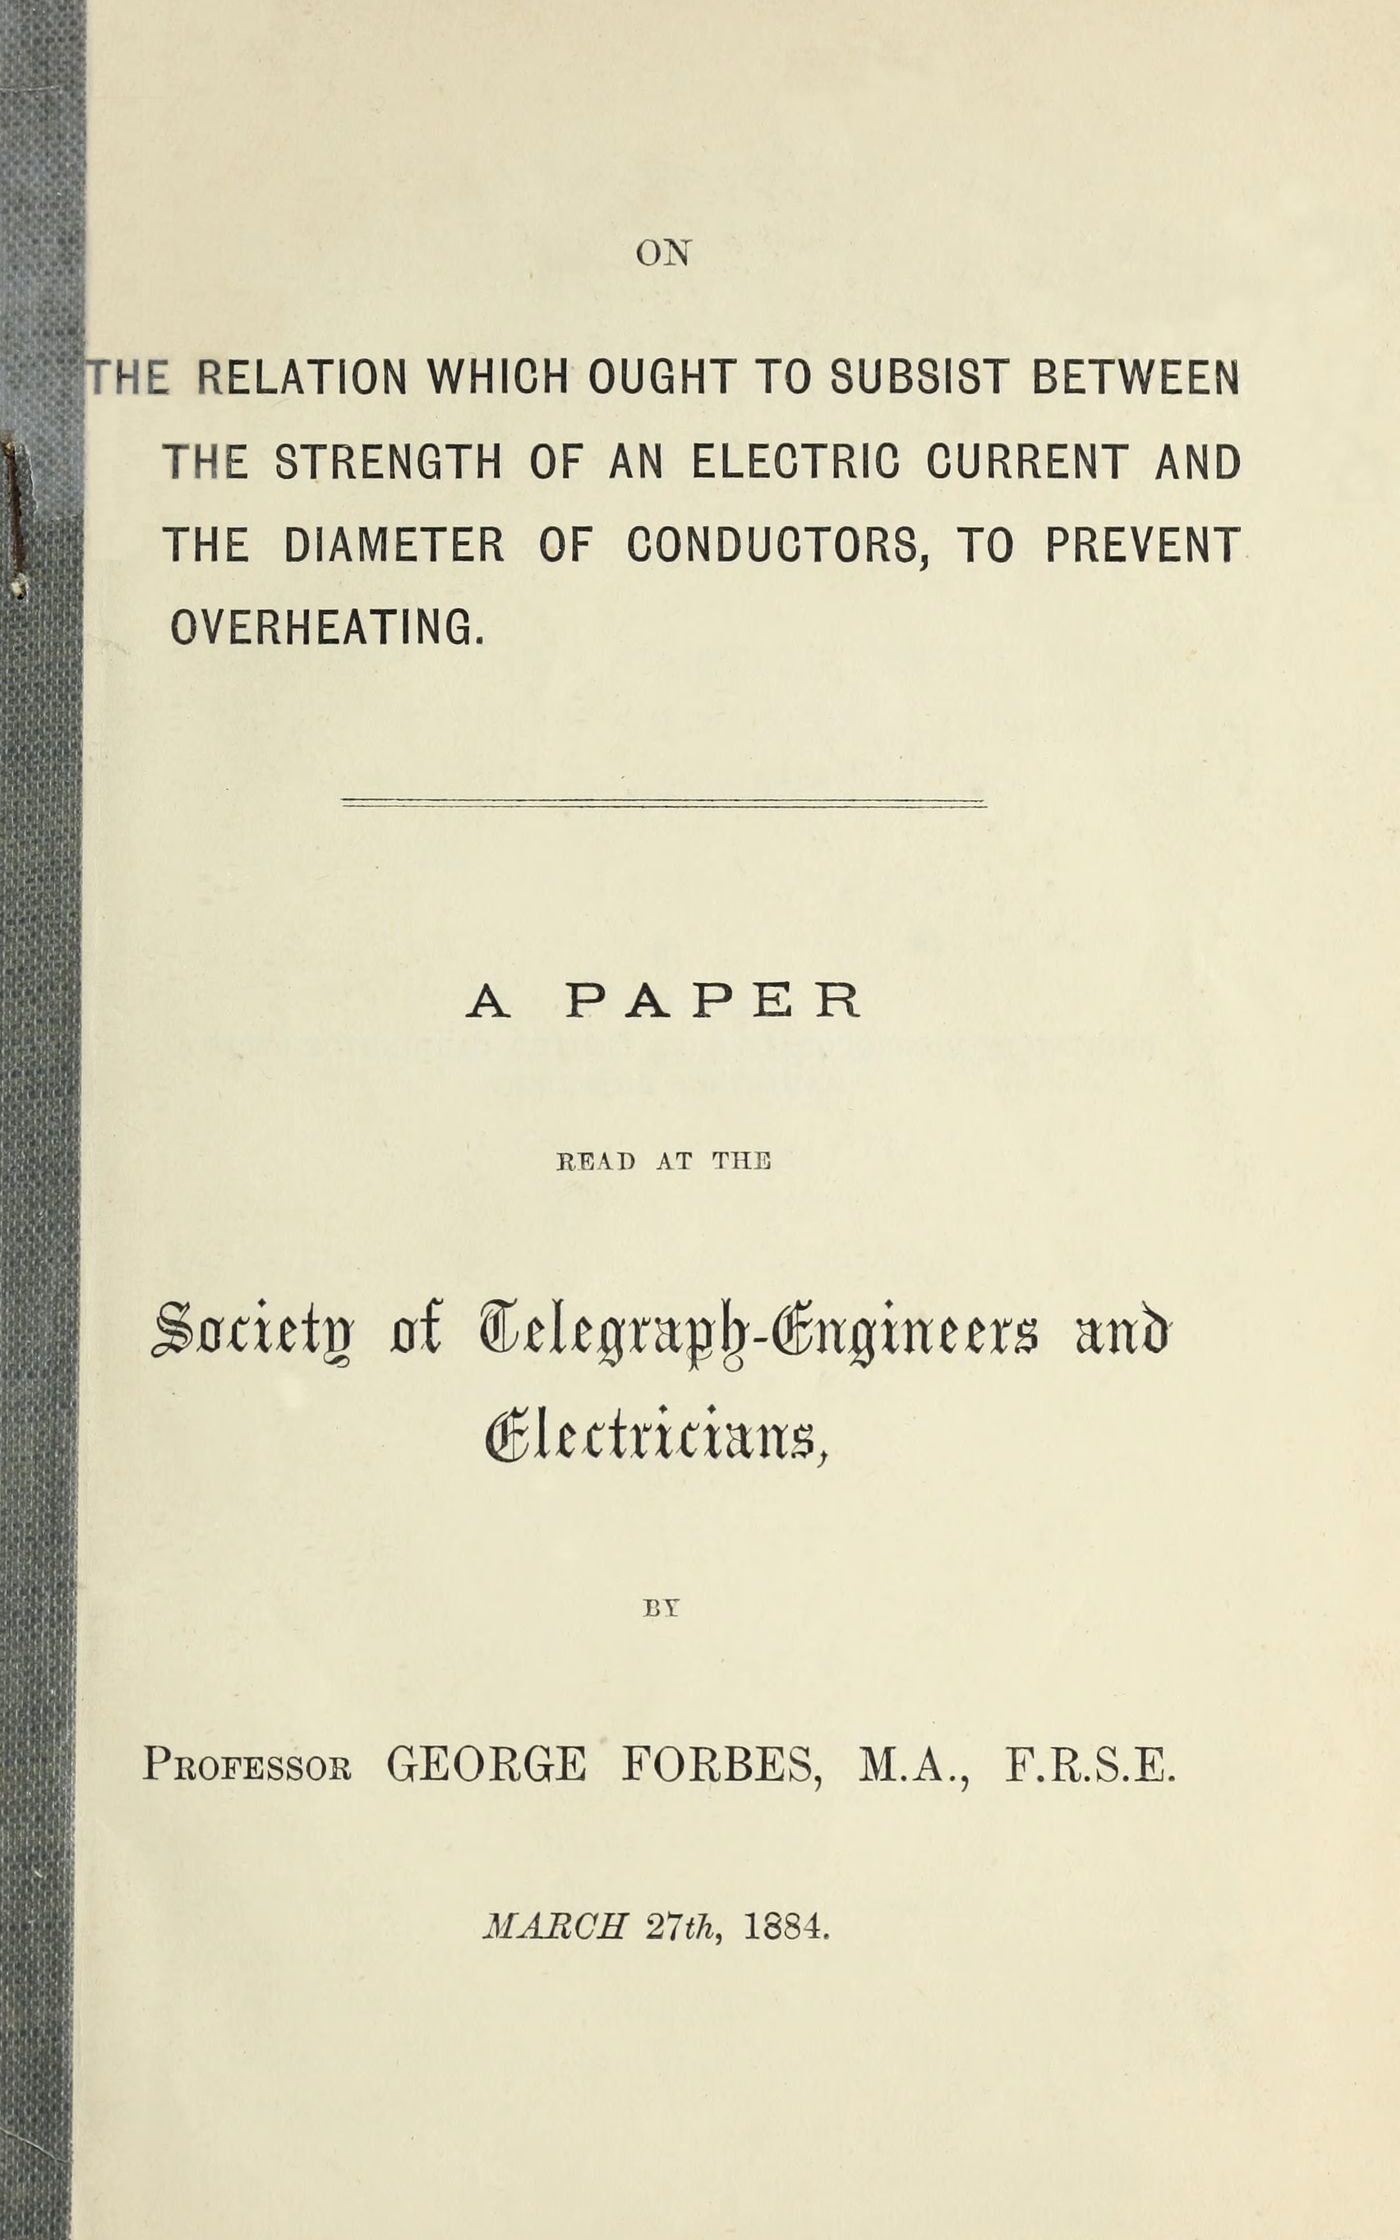
\includegraphics[width=0.999\textwidth,height=0.999\textheight,keepaspectratio]{cover.jpg}
\centering
\end{figure}
\restoregeometry

\newpage
\begin{PGtext}
\begin{center}
\large
\textbf{
The Project Gutenberg eBook of On the relation which ought to subsist between the strength of an electric current and the diameter of conductors, to prevent overheating by George Forbes
}
\end{center}
\InputIfFileExists{pgheader.tex}{}{}
\renewcommand*{\arraystretch}{1.5}
\begin{tabular}{p{2.5cm}>{\raggedright\arraybackslash}p{\dimexpr \linewidth-3.5cm}}
Title: &        On the relation which ought to subsist between the strength of an electric current and the diameter of conductors, to prevent overheating\\
Subtitle: &     A paper read at the society of telegraph-engineers and electricians, March 27th, 1884.\\
Author: &       George Forbes\\
Release Date: & November 18, 2022 [eBook \#69374]\\
Language: &     English\\
Produced by: &  The Online Distributed Proofreading Team at https://www.pgdp.net (This file was produced from images generously made available by The Internet Archive)\\
\end{tabular}
\vfill
\begin{center}
*** START OF THE PROJECT GUTENBERG EBOOK On the relation which ought to subsist between the strength of an electric current and the diameter of conductors, to prevent overheating ***
\end{center}
\end{PGtext}
%%-----File: 001.png-----%%
\pagestyle{fancy}
\fancyhf{}
\fancyhead[L]{}
\fancyhead[C]{\footnotesize ON THE PREVENTION OF OVERHEATING}
\fancyhead[R]{\thepage}
\setlength{\headheight}{14.5pt} % to avoid warnings
\mainmatter
\thispagestyle{empty}
\begin{center}
ON
\vspace*{.5cm}

{\blockfont\large
THE RELATION WHICH OUGHT TO SUBSIST BETWEEN
THE STRENGTH OF AN ELECTRIC CURRENT AND
THE DIAMETER OF CONDUCTORS, TO PREVENT
OVERHEATING.}

\vspace*{\fspace}
\doubleline
\vspace*{\fspace}
\large
\textls[300]{A PAPER} \\ [\fspace]
{\small READ AT THE} \\ [\fspace]
% :s gives final s rather than long s
\LARGE\textgoth{Society of Telegraph-Engineers: and
Electricians:,}

\vspace*{\fspace}
{\small BY } \\ [\fspace]
\large{\textsc{Professor} GEORGE FORBES, M.A., F.R.S.E.} \\ [\fspace]
\normalsize{\textit{MARCH} 27\textit{th}, 1884.}
\end{center}
%%-----File: 002.png-----%%
\newpage
\thispagestyle{empty}
\hspace{0pt} % needed so vfill fills from top
\vfill
\begin{center}
LONDON:

{\footnotesize PRINTED BY McCORQUODALE \& CO., LIMITED, CARDINGTON STREET,
HAMPSTEAD ROAD, N.W.}
\end{center}
\vfill
%%-----File: 003.png-----%%
\newpage
\thispagestyle{empty}
\begin{center}
ON
\vspace*{.5cm}

{\blockfont\large
THE RELATION WHICH OUGHT TO SUBSIST BETWEEN
THE STRENGTH OF AN ELECTRIC CURRENT AND
THE DIAMETER OF CONDUCTORS, TO PREVENT
OVERHEATING.}

\vspace*{1cm}
{\small BY } \\ [1cm]
{\large \textsc{Professor} GEORGE FORBES, M.A., F.R.S.E.} \\ [1cm]
\singleline
\vspace*{.5cm}
\begin{tabular}{l|l}
\textit{Sec.} 1. \textit{Introductory.} & \textit{Sec.} 4. \textit{Aerial \& Subaqueous Cables.}\\ [4pt]
\textit{Sec.} 2. \textit{Historical Summary.} &  \textit{Sec.} 5. \textit{Buried Conductors.}\\ [4pt]
\textit{Sec.} 3. \textit{Bare Conductors.} & \textit{Sec.} 6. \textit{Coils.} \\ [4pt]
\multicolumn{2}{c}{\textit{Sec.} 7. \textit{Conclusions.}} \\
\end{tabular}

\vspace*{0.5cm}
\singleline
\vspace*{.5cm}
\end{center}
\section*{Sec. 1. Introductory.}

The heating of conductors by the passage of an electric
current is injurious to the insulation if the conductor be
insulated, and may lead to risks from fire.

In small installations the heating of conductors is always
small, because of this fact—that if contractors were to lay down
wires so thin that overheating ensued, then we may be sure that
the resistance would be far too great for the capabilities of the
dynamo machine.
%%-----File: 004.png-----%%

But in large installations, currents of much greater density
being carried, the heating may be very great although the
resistance of the circuit is small; and it becomes a matter of the
utmost importance to know how the heating depends upon the
size of conductors and the current density.

I have searched in vain for experimental facts on a large scale,
and in absence of these have undertaken the mathematical
solution of the problem, and confirmed my results by a few
experiments on small currents, besides such isolated examples of
measurements of large currents as were available.

I have been at some trouble to determine carefully the nature
of conductors which would be required to carry a current capable
of supplying 100,000 lamps—say, 70,000 ampères. It may be said
that no such conductor would be required—that electricity will be
so carried in a network of conductors that in no part will the
current carried be excessive. It may further be said that high
tension currents will be used to charge accumulators in series,
scattered here and there over a district, and that, consequently,
small currents only will be required in the mains. To the latter
objection, I say that, to carry out some of the provisional orders
granted by the Board of Trade, the system of secondary batteries
being inadmissible, it will be necessary to carry through the
mains, current sufficient for all the lamps. To the former objection,
I say that the supply of gas gives us a valuable insight into
the similar progress which must be made in the supply of electricity.
The problems are remarkably similar, and a due attention
to this fact will save the pioneers of electricity much useless
expenditure of time, money, and thought. But in gas lighting
we carry enormous mains for distances of many miles from the
place of manufacture. Witness the huge 4-feet pipes laid
through this district last year, to carry gas from Wandsworth to
the City. There is no network of conductors here: it is found
necessary to carry in one main, gas enough to supply hundreds of
thousands of gas lamps. Let it be well noticed, also, that it
would be possible to force the gas at high pressure through narrow
tubes to fill and supply gas-holders spread about in different
parts of a district. The analogy to the proposed system of
%%-----File: 005.png-----%%
charging accumulators at high tension is perfect, and this leads
me to doubt very much whether the system which has not been
found advisable with gas is likely to be successful with electricity.

I still maintain that, to supply the electric light on a large
scale, we must face the problem of finding out what conductor
will carry a current of 70,000 ampères without overheating.

Now, in doing this we are going a step in advance of what has
been done before, just as (to cite, as example, a contemporary
engineering work), in designing the Forth Bridge, Messrs. Fowler
and Baker are extending the principles of bridge-making to
magnitudes hitherto unknown. Here the laws of the stability of
bridges are known, and, with experience on smaller bridges,
combined with laboratory tests of the strength of materials, a
sure advance can be made to the larger structure. It has been
my endeavour to find out whether, with the facts at our disposal
as to the smaller currents carried by smaller conductors, and the
laboratory experiments on the nature of our conductors and
insulators, we are in a position to propound laws which shall be a
guide to us in extending these principles to the construction of a
suitable conductor for very large currents, say, of 70,000 ampères.


\section*{Sec. 2. Historical Summary.}

In 1882 the Fire Risks Committee of this Society discussed
the question, and I believe I am right when I state that it was
seriously proposed as a rule, to prevent overheating of the wires,
that the permissible current should be so many ampères per
square inch section. I have often heard this error repeated. I
believe it has actually been adopted by the fire insurance companies
as a measure of safety, and a precise 1,000 ampères per
square inch has been given as the safe current. With regard to
the insurance companies, little harm has been done by this,
because they have had only small installations to deal with at
present, and, as above stated, there is practically no danger from
this cause; but it seems surprising that in one breath they
should tell contractors that in small installations they must not
raise the temperature of their conductors \(\xpa\frac{1}{10}\) of a degree, and
that in large installations they may make their conductors red-hot.
%%-----File: 006.png-----%%

As a matter of fact, in any installations, except very large
ones, the safe conductor ensures greater economy than the unsafe
one; and Sir William Thomson has done well\footnote
  {B. A. Reports, 1881, pp.\ 518 and 526.}
in fixing the size
of conductors by commercial considerations, when he showed
that the interest and depreciation on the cost of conductors
should equal the annual loss of horse-power in heating up these
conductors.

There is a limit above which this rule does not apply, because
the heating becomes so great that the insulation is injured. The
first person who, so far as I know, has taken notice of this, is
Mr.\ Cowling Welsch, in a table published by Messrs. E. \& F.
Spon. He fixes the limit at 2,700 ampères, but he does not state
what he considers to be the limiting temperature which is
tolerable, nor does he specify the nature of the insulation. His
facts seem to be taken from the tests of Messrs. Clark, Forde,
and Taylor (see next page.) Mr.\ T. Gray has also taken notice of
the failure of Sir William Thomson's law for high currents, in a
paper contributed to the \textit{Philosophical Magazine} in 1883, and
fixes the limiting value at 5,000 ampères.

I shall not take up the question of how Sir William Thomson's
rule is to be applied commercially. I have resolved in this
communication to confine myself to one point—the strength of
current which can be carried through a wire under different
conditions without overheating.

I find that two writers have worked at this subject from a
mathematical point of view, and each has worked out some concrete
examples. One of these is Mr.\ Day, of King's College,
whose useful little book, ``Electric Light Arithmetic,'' should be
studied by all learners. The other author is Mr.\ T. Gray. His
remarks on the subject appear in the \textit{Philosophical Magazine},
September, 1883. In discussing the question of bare wires, both of
these authors assume that the cooling effect is proportional to the
surface, and they make no reference to the variation from this law
which I pointed out in 1882 to the British Association, and which
has been confirmed by Mr.\ Preece. Mr.\ Day deals only with the
%%-----File: 007.png-----%%
case of a naked wire, in which he arrives at the theoretical law—\(\mathrm{(current)^2
\propto (diameter)^3}\)—which I published in 1882, but which
I also showed at that time to be contradicted by experiments on
a small scale. My own view of the matter is, that while, of course,
radiation is proportional to surface, convection is not so, but is
nearly constant for rectilinear wires of different diameters but the
same temperatures, and that with thin wires consequently convection
is the most important factor, but for thick wires radiation
proportional to surface is the ruling factor; hence the tables
which I have computed are correct for large diameters, but with
small wires greater currents may be safely carried.

Mr.\ Gray has also gone partially into the theory of an insulated
cable, and arrived at formulæ very similar to my own.

Some experiments were made by Messrs. Clarke, Forde, and
Taylor for the Indian and Oriental Electrical Storage and Works
Company, in the last year or two, and the results are published in
the \textit{Electrician} for April, 1883. The general conclusion arrived
at is, that up to 10 ampères it is safe to allow 1 ampère per 10
pounds of copper per mile, either with naked wire or with
insulated wires buried in sand, in the hot Indian climate. They
furnish the following table:—

\begin{table}[H]
\centering
\caption*{\textsc{CLARKE, FORDE, and TAYLOR'S TABLE.}}
\footnotesize
\begin{tabular}{|j{2.0}|j{2.0}|d|d|d|}
\hline
& & & & \\ [-5pt]
\multicolumn{1}{|c|}{B.W.G.} &
\multicolumn{1}{c|}{Diam. Mills.} &
\multicolumn{1}{m{2.3cm} |}{\centering Weight in lbs. per mile.} &
\multicolumn{1}{c|}{Ampères.} &
\multicolumn{1}{m{2cm} |}{\centering Lbs.\ per ampère.} \\ [10pt]
\hline
& & & & \\ [-10pt]
22 & 28 & 12.4 & 2.33 & 5.32 \\
21 & 32 & 16.2 &  2.84 & 5.70 \\
20 & 35 & 19.5 &  3.27 &   6.00 \\
19 & 42 & 28.0 &  4.3  &   6.5 \\
18 & 49 & 38.1 &  5.4  &   7.0 \\
17 & 58 & 53.3 &  6.9  &   7.7 \\
16 & 65 & 67.1 &  8.3  &   8.1 \\
15 & 72 & 82.5 &  9.6  &   8.6 \\
14 & 83 & 109.5 &  11.9 &    9.1 \\
13 & 95 & 143.0 & 14.56 & 10.0 \\
\hline
\end{tabular}
\normalsize
\end{table}
\normalsize
\vspace{1em}
\noindent No information is given as to the temperature which is considered
permissible.
%%-----File: 008.png-----%%

In the second supplement of the \textit{Electrician}, published in
March, 1883, a table was printed, supposed to give the currents
which could be safely worked through different thicknesses of
conductor. This table, however, was founded upon the assumption
that the safe-working current was proportional to the
sectional area, which is now well known to be far from the case.
I quote this simply as one example, out of many which has come
to my notice, of the same mistake being made by people who
ought to be better informed.

There are five primary cases of conductors which must be
treated separately—

\setlist{nosep}
\begin{itemize}[leftmargin=2cm]
\item[(1)] Overhead naked wires.
\item[(2)] Overhead cables.
\item[(3)] Subaqueous cables.
\item[(4)] Subterranean and embedded cables.
\item[(5)] Coils.
\end{itemize}

I have added the fifth case, of coils, because it is important in
the manufacture of dynamos and magnets.

Each of these classes has its own peculiarities. In all of them
heat is generated by the current, and this heat must be got rid
of. In case (1) it is got rid of solely by radiation and convection;
in the others partly by conduction, and in case (4) very largely
by absorption. In case (1) the maximum temperature is reached
almost immediately: in some of the other cases it may be many
hours before the final steady flow of heat sets in.

\section*{Sec. 3. Bare Copper Wires.}

Having convinced myself that the most satisfactory mode of
attacking the problem was to treat it in a strict mathematical
way, and being well aware that all the requisite data had been
obtained by previous experimenters, I determined to work out
practicable tables for the use of electricians from these data,
including both bare and insulated conductors. The first step was
to solve the following problem:—

Problem I.—\textit{To find the law connecting diameter, \(D\), of
conductor with that strength of current, \(C\), which raises its
%%-----File: 009.png-----%%
temperature by a fixed amount t° cent.\ above that of the surrounding
air.}

\begin{letlist}
\item[] Let R = the resistance in ohms of a cubic centimètre of the
substance of the conductor (= its specific resistance).
\item[] Let E = the heat radiated per second from a square centimètre
surface when the temperature of the surface is 1°
cent.\ above that of the surrounding air.
\end{letlist}

The radiation from the surface of 1 cm.\ length of the wire is
\(\pi\,D\,t\,E\), and this must equal the heat generated in 1 cm.\ length
of the substance \(= C^2 \cdot \dfrac{R}{\pi\left(\dfrac{D}{2}\right)^2}~\times\) (number of units of heat in 1
joule) \(= C^2 \cdot \dfrac{4 R}{\pi D^2} \times ·24\).\footnote
  {Everett's ``Units and Physical Constants.'' Joule's equivalent of a
Gramme centigrade heat unit \(= 4·2\times 10^7\) ergs, and one joule \(= 10^7\) ergs,
∴ ·24 = number of heat units in one joule.}

Whence
\[
\pi \,D \,t \,E = C^2 \frac{4 R \times ·24}{\pi D^2}
\]
and
\[
\label{eq:a}
C^2 = D^3 t\cdot\frac{\pi^2 E}{R \times 4 \times ·24}\tag{A}
\]

This shows that if the heat be lost by radiation, or by any
means which is proportional to the surface, then, in order to keep
all the wires of different diameters at the same temperature, we
must have the cubes of these diameters proportional to the squares
of the currents if the change of resistance with temperature be
neglected.

\textit{Example}:—To take, as a special example, the case of copper
we know that
\begin{tightcenter}
R = ·000001642 ohm\footnote
  {Maxwell's ``Electricity and Magnetism,'' Vol.\ I., last chapter.}
at 0° centigrade,
\end{tightcenter}
and increases ·38 per cent.\ per degree centigrade;
\begin{tightcenter}
E = ·000168 (polished), or ·000300 (blackened).\footnote
  {This is taken from D. McFarlane's experiments (\textit{Proceedings Royal Society,
Edinburgh}, 1872, p.\ 93), in which radiation took place from balls of considerable
size, and, consequently, convection played an unimportant part. If
the rise in temperature were 100° or more, it would become necessary to take
account of McFarlane's second and even third terms, depending on \(t^2\) and \(t^3\).}
\end{tightcenter}

To take an example, let C = 10 ampères; let the wire be
%%-----File: 010.png-----%%
No.\ 16 B.W.G. = 0·165 cm.; the rise of temperature comes out
\begin{align*}
t &= \text{21·2° C., polished,}\\
\shortintertext{or}
t &= \text{15·0° C., blackened.}
\end{align*}

\begin{sidewaystable}
\footnotesize
\captionsetup{justification=centering, font={footnotesize}}
\caption*{TABLE I.\\ \textit{Bare Copper Wires.—Current required to increase the temperature of a copper wire t° centigrade above the\\
surrounding air, the copper wire being bright polished or blackened.}}
\setlength{\bigstrutjot}{8pt}
\begin{tabular}{|d|j{4.0}|g|g|g|g|g|g|g|g|g|g|}
\hline
\multicolumn{2}{|@{}c@{}|}{\multirow{2}[4]{3cm}[0.2cm]{\centering Diameter in centimètres and mills. (thousandths of an inch).}} &
\multicolumn{10}{p{13cm}|}{\centering CURRENT IN AMPÈRES.\bigstrut} \\
\cline{3-12}
\multicolumn{2}{|c|}{} &
\multicolumn{2}{c|}{\(t\) = 1° C.\bigstrut} &
\multicolumn{2}{c|}{\(t\) = 9° C.} &
\multicolumn{2}{c|}{\(t\) = 25° C.} &
\multicolumn{2}{c|}{\(t\) = 49° C.} &
\multicolumn{2}{c|}{\(t\) = 81° C.} \\
\hline
\multicolumn{1}{|c|}{Cm.\bigstrut} &
\multicolumn{1}{@{}c@{}|}{Mills.} &
\multicolumn{1}{c|}{Bright.} &
\multicolumn{1}{c|}{Black.} &
\multicolumn{1}{c|}{Bright.} &
\multicolumn{1}{c|}{Black.} &
\multicolumn{1}{c|}{Bright.} &
\multicolumn{1}{c|}{Black.} &
\multicolumn{1}{c|}{Bright.} &
\multicolumn{1}{c|}{Black.} &
\multicolumn{1}{c|}{Bright.} &
\multicolumn{1}{c|}{Black.} \\
\hline
\setlength{\bigstrutjot}{2pt}
\bigstrut[t].1 &      40 &  1.0 &   1.4 &   3.0 &   4.1 &   4.8 &   6.6 &   6.5 &   8.9 &   7.9 &   11.0 \\
.2 &      80 &  2.8 &   3.9 &   8.3 &  11.5 &  13.5 &  18.7 &  18.3 &  25.3 &  22.4 &   31.0 \\
.3 &     120 &  5.2 &   7.2 &  15.3 &  21.2 &  24.9 &  34.4 &  33.5 &  46.4 &  41.2 &   57.0 \\
.4 &     160 &  8.0 &  11.0 &  23.6 &  32.7 &  38.3 &  53.0 &  51.7 &  71.5 &  63.4 &   87.8 \\
.5 &     200 & 11.1 &  15.4 &  33.0 &  45.7 &  53.5 &  74.1 &  72.2 &  99.9 &  88.6 &    123 \\
.6 &     240 & 14.6 &  20.3 &  43.4 &  60.0 &  70.3 &  97.4 &  94.9 &   131 &   116 &    161 \\
.7 &     280 & 18.5 &  25.6 &  54.6 &  75.6 &  88.7 &   123 &   119 &   165 &   147 &    203 \\
.8 &     310 & 22.6 &  31.2 &  66.7 &  92.4 &   108 &   150 &   146 &   202 &   179 &    248 \\
.9 &     350 & 26.9 &  37.3 &  79.6 &   110 &   129 &   179 &   174 &   241 &   214 &    296 \\
1.0 &    390 & 31.5 &  43.6 &  93.3 &   129 &   151 &   210 &   204 &   283 &   251 &    347 \\
2.0 &    790 & 89.2 &   123 &   264 &   365 &   428 &   593 &   577 &   799 &   709 &    981 \\
3.0 &   1180 &  164 &   227 &   485 &   671 &   787 &  1090 &  1061 &  1468 &  1303 &   1805 \\
4.0 &   1570 &  252 &   349 &   746 &  1035 &  1211 &  1675 &  1633 &  2260 &  2006 &   2776 \\
5.0 &   1970 &  353 &   488 &  1043 &  1444 &  1692 &  2343 &  2283 &  3160 &  2802 &   3880 \\
6.0 &   2360 &  463 &   642 &  1371 &  1898 &  2225 &  3080 &  3000 &  4154 &  3685 &   5100 \\
7.0 &   2760 &  584 &   808 &  1728 &  2392 &  2803 &  3882 &  3781 &  5233 &  4642 &   6426 \\
8.0 &   3150 &  714 &   988 &  2110 &  2922 &  3422 &  4741 &  4620 &  6396 &  5671 &   7850 \\
9.0 &   3540 &  851 &  1178 &  2519 &  3486 &  4088 &  5659 &  5511 &  7630 &  6769 &   9370 \\
10.0 &  3940 &  997 &  1380 &  2950 &  4084 &  4788 &  6626 &  6455 &  8935 &  7926 &  10973 \\
34.4 &  \dots & \dots & \dots & \dots & \dots & \dots & \dots & \dots & \dots & \dots & 70000 \\
\hline
\end{tabular}
\end{sidewaystable}
\normalsize

The accompanying Table I. has been computed from the formula
obtained above:
\[
C^2 = D^3 t\cdot\frac{\pi^2 E}{4 R \times 0·24}
\]
%%-----File: 011.png-----%%
\begin{align*}
C &= \text{current (ampères).}\\
D &= \text{diameter of wire (centimètres).}\\
t &= \text{excess of temperature (centigrade) above air.}\\
E &= \text{coefficient of radiation and convection.}\\
R &= \text{specific electrical resistance (ohms).}\\
.24 &= \text{number of gramme-centigrade heat units in a watt.}\\
&\text{Temperature of the air assumed 20° C.}\\
R &= 0·000001642 \xp\left(1 + \dfrac{·38 t}{100}\right)\text{.}\\
E &= \text{·000168 for polished, ·00032 for blackened, copper.}\\
\end{align*}
It gives the rise in temperature in bare copper
wires with different currents. In computing with this formula, it
must be noticed that the value of R, the specific resistance, varies
with the temperature. The resistance at 0° C. is 1642, as stated
above. At the temperature of the air (which may be taken at
20° C.) it is 1736, and at any temperature which is \(t\)° above 20° C.
the resistance is \(1642\,(1 + ·0038\,(t + 20))\). This change of resistance
produces a change of 15 per cent.\ in the current which can
be carried at the higher temperatures.

The effects of temperature in altering the resistance are continually
cropping up in our application of theory to practice, and
the following very striking experiment is worth recording:—

I have been informed by Mr.\ H. Edmunds that he made experiments
with wires \(\xpa\frac{1}{32}\) inch diameter, flattened out to various widths,
through which he passed the current from a machine, the E.M.F.
being the same in all the experiments. In the form of wire \(\xpa\frac{1}{32}\)
inch diameter, it was heated to a bright colour; when flattened to
\(\xpa\frac{1}{16}\) and \(\xpa\frac{1}{8}\) inch width, it lost luminosity; and so on until, when used
in a strip \(\xpa\frac{1}{2}\) inch wide, it kept pretty cool, and fairly stopped the
engine. Here we see that the resistance of the wire and all the
strips was the same at any constant temperature, but the surface
for cooling by radiation and convection was greater with the wider
strips. This explains why the wider strips were cooler than the
narrower ones, and still more than the wire. Lastly, the resistance
is trebled at a temperature which makes the metal barely luminous,
and is enormously increased at a bright heat. Hence, in the cases
%%-----File: 012.png-----%%
where there was bright luminosity, there was high resistance and
less current. The wide strip, being the coolest, had most current,
and used up most work, and so stopped the engine.

In the above table (as in the others which follow it), the current
specified heats the wire to the degree stated only when
steadily applied. A much more powerful current might be used
for a very short time at intervals, as in signalling for railways.

The only doubt of the accuracy of the table can come from
a doubt as to the accuracy of McFarlane's experiments, which
were made in Sir William Thomson's laboratory, or in the
extension of his results to surfaces of different dimensions. On
this matter I have a few remarks to make.

1. The value which McFarlane found for the loss of heat
per second per degree difference of temperature between the
metal and the enclosure increased from \(t\) = 5° C. to \(t\) = 60° C.
in the ratio \(178 : 226\) for polished copper. I have used the
value 178 in calculating the above table, so that the current
which can be carried with the copper in any state of oxidation,
or dirt, is certain to lie between the two values given in the table
under \textit{bright} and \textit{blackened}.

2. The only experiments with which I can compare Mr.\
McFarlane's are those by the late Mr.\ Nichol, published by
Professor Tait in the \textit{Proceedings Royal Society, Edinburgh},
1869-70, p.\ 207. The following table gives the comparison.

\begin{table}[H]
\footnotesize
\smallskip
\hangind{\textit{Loss of heat} (\textit{per sq.\ cm.\ per second per degree centigrade difference of temperature})
\textit{from copper in air at atmospheric pressure in blackened enclosure at constant
temperature} (8° \textit{C. in Nichol's experiments}), \textit{for various differences of temperature}:—}
\smallskip
\begin{tabular}{|d|e|e||d|e|e|}
\hline
\multicolumn{3}{|c||}{Polished.\strutb} &
\multicolumn{3}{c|}{Blackened.} \\
\hline
\multicolumn{1}{|c|}{\multirow{2}{2.1cm}[-0.3cm]{\centering Difference of temperature.}} &
\multicolumn{2}{p{3.5cm}||}{\centering \sstrut Loss per sq.\ cm.\ per sec.\ per degree.\estrut} &
\multicolumn{1}{c|}{\multirow{2}{2.1cm}[-0.3cm]{\centering Difference of temperature.}} &
\multicolumn{2}{p{3.5cm}|}{\centering Loss per sq.\ cm.\ per sec.\ per degree.}\\
\cline{2-3} \cline{5-6}
& \multicolumn{1}{c|}{McFarlane.\strutb} &
\multicolumn{1}{c||}{Nichol.} &
& \multicolumn{1}{c|}{McFarlane.} &
\multicolumn{1}{c|}{Nichol.} \\
\hline
\multicolumn{1}{|c|}{} & & &
\multicolumn{1}{c|}{} & & \\ [-10pt]
\multicolumn{1}{|c|}{Degrees.} & & &
\multicolumn{1}{c|}{Degrees.} & & \\
10.0 & .000176 & \edots  & 10.0 & .000266 & \bdots  \\
12.5 & \bdots  & .000198 & 12.5 & \bdots  & .000364 \\
15.0 & .000193 & \edots  & 19.3 & \bdots  & .000331 \\
15.3 & \bdots  & .000182 & 20.0 & .000289 & \bdots  \\
20.0 & .000201 & \edots  & 30.0 & .000306 & \bdots  \\
21.6 & \bdots  & .000175 & 33.6 & \bdots  & .000320 \\
30.0 & .000212 & \edots  & 40.0 & .000319 & \bdots  \\
32.5 & \bdots  & .000173 & 42.2 & \bdots  & .000322 \\
40.0 & .000220 & \edots  & 50.0 & .000326 & \bdots  \\
42.5 & \bdots  & .000173 & 53.2 & \bdots  & .000328 \\
50.0 & .000225 & \edots  & 60.0 & .000328 & \bdots  \\
55.8 & \bdots  & .000177 & & & \\
60.0 & .000226 & \edots  & & & \\
\hline
\end{tabular}
\normalsize
\end{table}

A comparison of the results of McFarlane and Nichol shows
that they agree generally as well as could possibly be expected,
so far as the term which depends on the first power of the
temperature in the expression
\[
\text{loss of heat} = A\,t + B\,t^2 + C\,t^3 + \cdots
\]
is concerned, but that in the comparatively unimportant second
term McFarlane makes B negative, and Nichol makes it sometimes
positive and sometimes negative. The general conclusion
is that we can trust safely to the first term, but that we must not
push the application to extremely high temperatures.

3. Both the above sets of experiments were made upon
masses of metal some centimètres in diameter, and the conclusion
seems warrantable that with such masses my formula is accurate.
%%-----File: 013.png-----%%
I state this now, because I have next to show that the law does not
extend to small masses where convection plays a more important
part than radiation. My impression is that thin wires lose their
heat chiefly by convection when free in the air, but larger masses
chiefly by radiation.

I worked at the subject experimentally in 1881 and the
following years. My results were published in the \textit{British
Association Reports}, 1882; \textit{Annales de l'Electricité}, 15th October,
1882; the \textit{Electrician}, 1882, September, and 1883, February.

My first object in those experiments was to test the correctness
of the following considerations:—When a current passes
through a wire keeping up a constant temperature, the heat
developed by the current over a given length is equal to that
lost by radiation, convection, and conduction. It seemed right
to suppose that at a fixed temperature this cooling varies as the
%%-----File: 014.png-----%%
surface, \ie, as the diameter of the wire. The heat generated
by the law of Joule varies as \(C^2 R\) or \(\dfrac{C^2}{D^2}\), where C = the current,
R the resistance, and D the diameter of the wire.

Whence
\begin{align*}
\frac{C^2}{D^2} &= a D~(a\text{ being a constant}),\\
\shortintertext{and}
C &= a D^{\tfrac{3}{2}.}
\end{align*}

To verify the exactness of this law, I experimented on several
wires of different diameters but the same conductivity. Each
wire was thinly coated with beeswax, whose melting point was
58° C., the temperature of the room being 18° C\@. A current
was passed through one of these wires, and resistances were slowly
and gradually removed from the circuit, until the current heated
the wire so as to melt the wax. The angle of deflection of the
tangent galvanometer was then read off, to give the intensity of
the current. The same operation was repeated on the other wires,
and the following table gives the results obtained:—

\footnotesize
\vspace{1em}
\begin{center}
\begin{tabular}{|h|h|h|h|h|}
\hline
 & & & & \\ [-5pt]
\multicolumn{1}{|c|}{D} &
\multicolumn{1}{c|}{C} &
\multicolumn{1}{c|}{\(\dfrac{C}{D}\)} &
\multicolumn{1}{c|}{\(\dfrac{C}{D^{\frac{3}{2}}}\)} &
\multicolumn{1}{c|}{\(\dfrac{C}{D^2}\)} \\ [10pt]
\hline
 & & & & \\ [-10pt]
\multicolumn{1}{|c|}{Mm.} & & & & \\
0.58 & 0.984 & 1.696 & 2.229 & 2.924 \\
1.22 & 2.304 & 1.888 & 1.709 & 1.548 \\
1.58 & 3.026 & 1.915 & 1.523 & 1.212 \\ [8pt]
\hline
\end{tabular}
\end{center}
\normalsize
\vspace{1em}

If \(C \propto D^{\frac{3}{2}}\), the quotient \(\dfrac{C}{D^{\frac{3}{2}}}\) should be constant for all the
wires. If, as some have supposed, \(C \propto D^2\), the quotient \(\xp\dfrac{C}{D^2}\)
should be constant. If, lastly, \(\dfrac{C}{D}\) is more nearly constant, as is
seen to be the case, the law is that the current varies more nearly
as the diameter.

Within the last few days I have come across some tests which
I had made in 1881, on five thicknesses of lead wire, to find the
current required to fuse them. I found that this depended upon
the length of the specimen. The reason is that the ends of the
wire are clamped by cold metal, which absorbs the heat, and so a
%%-----File: 015.png-----%%
greater current is carried without fusion with short specimens
than with long ones. I give the results for what they are worth.

\begin{table}[H]
\centering
\footnotesize
\caption*{\textit{Fusing Currents for Lead Wires.}}
\renewcommand*{\arraystretch}{1.01}
\begin{tabular}{|c@{}j{1.2}|j{1.3}|j{2.3}|}
\hline
 & & & \\ [-6pt]
\multicolumn{2}{|c|}{Diameter.} &
\multicolumn{1}{c|}{Length.} &
\multicolumn{1}{c|}{Fusing Current.} \\ [8pt]
\hline
 & & & \\ [-6pt]
& \multicolumn{1}{c|}{Mm.} &
\multicolumn{1}{c|}{Mètre.} &
\multicolumn{1}{c|}{Ampères.} \\
& 0.55 & 0.025 &  0.78 \\
& 0.78 & 0.025 &  0.937 \\
& 0.94 & 0.025 &  1.125 \\
% 2nd parameter * avoids overfull hbox
% use 1.5 rows rather than 2 to avoid overfull vbox
\ldelim\{{2}{*}
& 1.03 & 0.025 &  8.2 \\
& 1.03 & 0.225 &  6.0 \\
\ldelim\{{5}{*}
& 1.28 & 0.300 &  9.5 \\
& 1.28 & 0.150 & 12.37 \\
& 1.28 & 0.075 & 12.75 \\
& 1.28 & 0.050 & 13.5 \\
& 1.28 & 0.025 & 16.87 \\ [8pt]
\hline
\end{tabular}
\normalsize
\end{table}

These measurements were not made by myself, and I cannot
vouch for any very great accuracy. One fact which we learn from
them is, that in such experiments, with wires about 1 millimètre
thick, the length in experiments of this nature should be not less
than 30 centimètres, or, generally, the length should be 300 times
the diameter. The effect of using short wires is especially shown
with the thicker ones, the experiments on which show that a
large quantity of heat is carried off by thermal conduction to the
massive cooling terminals.

Taking the case of a long wire, let us see how far it gives us
reason to believe in the applicability of the formulæ of this
memoir to practical cases. A lead wire, 1·28 millimètre diameter
and of considerable length, was heated to the temperature of
fusion with a current of 9·5 ampères, and one of 1·03 millimètre
diameter, with a current of 6·0: let us find the theoretical current
required.

By referring to Problem I., we see that the heat generated per
second in one centimètre length of the substance \(= C^2 \dfrac{R}{\pi \left(\dfrac{D}{2}\right)^2} \times ·24\) where
\begin{description}[leftmargin=1em]
\item[]C = current in ampères,
\item[]R = specific resistance in ohms,
\item[]D = diameter.
\end{description}
%%-----File: 016.png-----%%
\vspace{1em}
Now R\footnote{Jenkin: Cantor Lectures.} = 19,850 at 0° C. for lead in C.G.S. units.\\
% hack alignment (footnote doesn't work in maths)
\phantom{Now R* }= 44,751 at 327° in C.G.S. units,\\
\phantom{Now R* }= ·000044751 in ohms.

\noindent
The melting temperature of lead being 327° C.\footnote
{Balfour Stewart: ``Elementary Treatise on Heat,'' p.\ 88.}, or, say, 310° C.
above the surrounding air,\\
∴ heat generated \(= C^2\dfrac{·000044751 \times 4}{\pi D^2} \times ·24 = ·0000570 \dfrac{C^2}{D^2} \times ·24\).

\vspace*{.4cm}
Referring to McFarlane's experiment, I find that 60° C. excess
of temperature gives a loss of heat per square centimètre per
second = ·01356 gramme centigrade heat units with polished
copper, and that the loss is nearly proportional to the temperature.
This would give ·07006 for 310° C.

The surface of one centimètre length of the first wire is
\[\pi \times ·128 = ·402,\]
and of the second it is
\[\pi \times ·103 = ·324;\]
and the loss of heat is in the first wire
\[·07 \times ·402 = ·02814,\]
in the second
\[·07 \times ·324 = ·02268,\]
and this must equal the heat generated as given above, viz.—
\begin{align*}
 &= ·0000570 \times ·24\,\frac{C^2}{D^2} \\
 &= ·00001368\,\frac{C^2}{D^2} \\
 &= ·000848\,C^2 \ \text{for the first wire,} \\
\text{and } &= ·001290\,C^2 \ \text{for the second wire;}
\end{align*}
whence for the first wire
\[C^2 = \frac{·02814}{·000848}\]
and for the second
\[C^2 = \frac{·02268}{·001290}\]
which gives us 5·8 and 4·2 ampères theoretically in place of
9·5 and 6·0 respectively, as found by experiment. This only shows
%%-----File: 017.png-----%%
that McFarlane's constant does not apply to high temperatures,
and that the loss of heat is then much greater than in direct proportion
to the temperature.

The only extensive experiments on the subject, with which I
am acquainted, have been made by Mr.\ W. H. Preece, and the
results are about to be communicated to the Royal Society. He
has been kind enough to show me his experimental results, in order
that I might be able to bring before you a comparison with my
own results.

He measured the current which was just sufficient to melt
platinum wires of different sizes, and he also measured the current
which is just sufficient to make wires luminous. The results
obtained by Mr.\ Preece confirm my experiments, and show that
with small wires the \((\mathrm{current})^2\) is more nearly proportional to the
\((\mathrm{diameter})^2\) than to the \((\mathrm{diameter})^3\).

\section*{Sec. 4. Aerial and Subaqueous Cables.}

We now come to the case of insulated conductors. There
are two cases which can be taken together—aerial and subaqueous.
The mathematical treatment of these is, however, not
quite the same. In the subaqueous cable we may assume that the
outside of the insulator remains at the temperature of the water.
In an aerial line it sometimes happens that the insulator is so thin
that its outside becomes quite hot. The mathematical view of
this case is nearly the same as that of a copper conductor covered
with lampblack, which case has already been treated.

Problem II.—\textit{A conductor of radius \(r_{1}\) is surrounded with an
insulator to an outer radius \(r_{2}\). If the ratio \(\dfrac{r_2}{r_1}\) remains constant,
it is required to find the way in which the current \(C\) must vary
with radius \(r_{1}\), so that the temperature of the wire shall be \(t_{1}\)
degrees cent.\ above that of the outside of the insulator.}

\begin{letlist}
\item[] Let R, as before, be the specific electrical resistance of the
conductor in ohms, and let K be the thermal conductivity
of the insulator.
\item[] Let H be the heat which is generated per second by the
current in a length of one centimètre of the conductor.
\end{letlist}
%%-----File: 018.png-----%%
Then H is also the heat which flows per second radially out of the
insulator per centimètre of length. Imagine the insulator to be
made up of a number of concentric cylinders, and let the radius
of one of them be \(r\) and the thickness \(\delta\,r\), then the surface of one
centimètre length of this cylindrical shell is \(2 \,\pi \,r\); and if \(- \delta \,t\)
be the difference of temperature, we have, from Fourier's definition
of conductivity,
\[
H = -K \cdot \frac{2 \,\pi \,r \cdot \delta \,t}{ \delta \,r}
\]

If we integrate this between the limits \(r = r_{1}\) and \(r = r_{2}\),
the difference of temperatures at these points being \(t_{1}\), we find
that
\[
\log._{e} \frac{r_{2}}{r_{1}} = \frac{2 \,\pi \, K}{H} t_{1}
\]

Now we also know, from Joule's law, that the heat generated
in one centimètre length of the conductor is
\begin{gather*}
H = \frac{4 \,C^2 \,R}{\pi \,D^2_{1}} \times \text{(number of heat units in one joule = 0·24).}\\
\text{∴ } \log._{e} \frac{r_{2}}{r_{1}} = \frac{\pi^2 \, K \, D^2_{1}}{·48 \, C^2 \, R} t_{1}\\
C = \sqrt{ \frac{\pi^2 \, D^2_{1} \cdot K \,t_{1}}{ ·48 \, R \,\log._{e} \dfrac{D_{2}}{D_{1}}}}\tag{1}
\end{gather*}
It appears from this, that when the ratio \(\xp\dfrac{D_{2}}{D_{1}}\) is constant, the current
must vary as the radius of the conductor to produce a constant
difference of temperature between the inside and outside of the
insulator. But it would be comparatively useless to tabulate the
data from this formula, for with aerial cables we must take note
of the excess of temperature of the outside of the insulator over
the surrounding air. Call this excess \(t_{2}\). Then, from the method
pursued in the investigation for bare wire, E being, as before, the
coefficient of radiation and convection, the flow of heat is
\[
= \pi \, D_{2} \,t_{2} \, E
\]
but it is also
\[
= \frac{2 \,\pi \, K \,t_{1}}{\log._{e}\dfrac{D_{2}}{D_{1}}}
\]
%%-----File: 019.png-----%%
whence
\[
\frac{t_{1}}{t_{2}} = \frac{D_{2} \, E \cdot \log._{e} \dfrac{D_{2}}{D_{1}}}{2 \, K}
\]
putting E = ·0003 (see above) and K = ·0005
\begin{gather*}
\frac{t_{1}}{t_{2}} = \frac{3}{10} D_{2} \log._{e} \frac{D_{2}}{D_{1}} \tag{2}\\
\text{∴ } t = t_{1} + t_{2} = t_{1} \cdot \frac{10 + 3 \, D_{2} \, \log._{e} \dfrac{D_{2}}{D_{1}}}{3 \,D_{2} \, \log._{e} \dfrac{D_{2}} {D_{1}}} \tag{3}
\end{gather*}
and from (1)
\[
C = \bigsurd \left\{ \frac{ \pi^2 \, K \, D^2_{1}} {·48 \, R} t \times \frac {3 \, D_{2}}{10 + 3 \, D_{2} \, \log._{e} \dfrac{D_{2}}{D_{1}}} \right\}
\]

This formula is one of great interest. From it we can
calculate directly the value of the current or the rise in temperature,
when the other quantities are fixed; and all the
problems in connection with such cables as are discussed in
this memoir can be dealt with by the help of the same formula.
There is another matter of great practical importance which it
enables us to solve. We can compare it with the \hyperref[eq:a]{formula (A) on
page \pageref{eq:a}}, for bare copper wire. Call \(I\) and \(I'\) the currents in
bare and insulated wires, which with the same value of D give
also the same value of \(t\).

Assume E = ·0003 for insulation, and \(E'\) = ·0002 for copper.
\begin{align*}
\frac{I^2}{I'^2} & = \frac{D^3 \, t \cdot \dfrac {\pi^2 \, E'}{R \times 4 \times ·24}}{\dfrac{D^2_{1} \, D_{2} \, \pi^2 \, K \, E \cdot t}{2 \times ·24 \times R} \cdot \dfrac{1}{2 \, K + E \cdot D_{2} \, \log._{e} \dfrac{D_{2}}{D_{1}}}}
\\&= \tfrac{2}{3} \times  \frac{D^3}{D^2_{1} \, D_{2}} \cdot \frac{1}{2 \, K} \cdot \left(2 \, K + D_{2} \, E \, \log._{e} \frac{D_{2}} {D_{1}}\right)
\\&= \tfrac{2}{3} \cdot \frac{D^3}{D^2_{1} \, D_{2}} \cdot \tfrac {1}{2} \cdot \left(2 + \left\{\frac{E}{K} = \tfrac{3}{5}\right\} \cdot D_{2} \, \log._{e} \frac{D_{2}}{D_{1}}\right)
\end{align*}
and \(D = D_{1}\).

Thus we find that \(I\) is greater or less than \(I'\), according as
\[
2 \, D_{1} \left(2 + \tfrac{3}{5} \, D_{2} \log._{e} \frac{D_{2}}{D_{1}}\right) \text{is} \gtrless 6 \, D_{2}.
\]
%%-----File: 020.png-----%%
Take as special cases (1) \(D_{2} = 2 D_{1}\) and (2) \(D_{2} = 4 D_{1}\).
Then \(I\) is \(\gtrless I'\), according as
\begin{align*}
   &(1)~4 + \tfrac{6}{5} D_{2} \times ·693 \text{ is } \gtrless 6 \times 2, \\
\text{and } &(2)~4 + \tfrac{6}{5} D_{2} \times 1·386 \text{ is } \gtrless 12 \times 2,
\end{align*}
\ie, according as
\begin{align*}
&(1)~D_{2} \text{ is } \gtrless \frac{6 \times 2 \times 5 - 20}{6 \times ·693} \gtrless 9·6, \\
\text{and } &(2)~D_{2} \text{ is } \gtrless \frac{12 \times 2 \times 5 - 20}{6 \times 1·386} \gtrless 12·0,
\end{align*}
\begin{align*}
\text{or } &(1) \text{ as } D_{1} \text{ is } \gtrless 4·8 \text{ centimètres},\\
\text{and } &(2) \text{ as } D_{1} \text{ is } \gtrless 3·0 \text{ centimètres.}
\end{align*}
If different values of E and K are adopted, these values will
vary proportionally to \(\xp\dfrac{K}{E}\), here assumed to be \(\tfrac{3}{5}\).

We have now arrived at a most important result, viz., that an
insulated wire carries a greater current without overheating than
a bare wire, if the diameter be not very great. Assuming the
diameter of the cable to be twice that of the conductor, a greater
current can be carried in insulated cables than in bare wires up
to 4·8 centimètres diameter of conductor. But if the insulated
cable have a diameter four times that of the conductor, this is the
case up to 3·0 centimètres diameter of conductor.

When the thickness of insulation is made very great, the limiting
size of conductor which favours the insulated wire is shown
below:—

\vspace*{.4cm}
\footnotesize
\begin{tabular}{j{2.0} c p{1.6cm} j{1.1}@{ }c c}
\multicolumn{1}{c}{\(\dfrac{\text{Diameter of insulator.}}{\text{Diameter of conductor.}}\)} & &
\multicolumn{4}{m{5cm}}{\centering Limiting diameter of conductor which favours insulation.} \\ [10pt]
2 & \dots & & 4.8 & cm. &\\
4 & \dots & & 3.0 & „ &\\
6 & \dots & & 2.5 & „ &\\
8 & \dots & & 2.2 & „ &\\
10 & \dots & & 2.0 & „ &\\
100 & \dots & & 1.0 & „ &\\
\end{tabular}
\normalsize
\vspace*{.4cm}

\noindent
I venture to express the conviction that these results must
be looked upon as very surprising. It was hardly to be
expected that, by surrounding a copper wire with a bad conductor
of heat, we could in any case increase the strength of
%%-----File: 021.png-----%%
current which it will carry without overheating. Yet such is
clearly the case; and the general explanation of it is that by so
doing we increase the surface from which radiation and convection
take place. When, however, we have to deal with large currents
in large conductors, and the thickness of insulating material is
increased in the same ratio, the heat finds greater difficulty in
penetrating so thick a mass, and the insulation becomes objectionable
from its bad heat-conducting properties, so as to lead us to
the result that the bare wire carries more current than the
insulated one without overheating, when the diameter is great.

It has been supposed by some persons that heat will escape
far more freely through insulating materials, owing to their
sometimes being diathermanous, and allowing heat to be radiated
through them. Now, in opposition to this view, I must say that
very few such substances are diathermanous, and very seldom are
they sufficiently homogeneous to allow the possibility of direct
radiation through their mass.

Before I go on with what I have to say, I must now pause to
make a few remarks on the problem which has just been solved.

1. \textit{Permanent State.}—The definition of Fourier, which has
been made the basis of the calculations, has reference to the case
only when heat has been steadily supplied for some time, so that
the gradation of temperatures from the hot interior and the cool
exterior has reached what is called the permanent state. The
time which is required to attain this state varies with the conditions
of the case. With an insulated cable this time increases
with the thickness of the insulating material. It may often
happen that many hours must elapse before this state is arrived
at, \ie, before the calculations of the present part of my paper
can be applied. It must be noticed that previous to the establishment
of the permanent state the heating effect is less injurious;
so that in all cases where there is a considerable amount of
insulating material the current may, during the first working
hours, be considerably in excess of what has been calculated out
here as the working current. The reason of this is, that during
this preliminary stage the heat is used up in raising the temperature
of the insulating material, which serves to cool the
conductor.
%%-----File: 022.png-----%%

2. \textit{Specific Heat.}—This leads me to my second remark about
the above calculations, viz., the influence of specific heat of the
insulator. It has been explained that, after the permanent state
has set in, the heat which is generated in the conductor all passes
through the insulator to the external air. But previous to that
time the heat generated is partly used up in raising each layer of
the insulator up to the temperature which it must have when in
permanent state. The quantity of heat used up in this way
depends upon the specific heat of the insulator. The specific heat
is the number of units of heat required to raise the temperature
of one gramme of the material 1° C\@. This quantity is known for
a large number of substances.

A patent has been taken out for resistances of fine wire through
which large currents can be made to pass without undue heating,
by embedding the wire in cement or plaster of Paris. The cooling
effect of the plaster of Paris is dependent upon its specific heat,
and is only temporary. After a very long run of a current through
such a conductor, the heating may become greater than in air;
and, if the temperature be that of red heat, the plaster becomes a
good enough conductor to lower the resistance of the combination
so as to make it useless.

I have known of cases where much larger currents have been
carried through cables than would be possible by the formula: it
is probable in these cases that the current was not continued
long enough for the permanent distribution of the temperature to
be arrived at. Hence the wire carried a larger current without
overheating.

3. Let us form some estimate of the work which is required
to heat the insulator to its permanent condition. The exact
solution of this problem is troublesome, so we must be content
with a very general view of the question. If \(r_{1}\) and \(r_{2}\) be the
radii of the interior and exterior respectively of the insulator, the
mass of this material in a centimètre length is \(\pi\,(r^2_{2} - r^2_{1})\). Its
weight is \(w\,\pi\,(r^2_{2} - r^2_{1})\) when \(w\) is the specific gravity of the insulator.
The heat required to raise its temperature 1° C. is \(c\,w\,\pi\,(r^2_{2} - r^2_{1})\)
when \(c\) is the specific heat of the material. I can find
no determination of the specific heat of gutta percha, but, by the
%%-----File: 023.png-----%%
analogy of the substances which it most resembles, it is probably
about 0·2. We may take this value for the present, remembering
that it is desirable to have experiments made upon all the substances
used as insulators, so as to know their specific heats. The
density of gutta percha is about 1·0. If we take, as an example,
the data derived from an experiment in which C = 500, \(r_{1} = ·625\),
\(r_{2} = 5\), we find
\begin{align*}
c\,w\,\pi\,(r^2_{2} - r^2_{1}) &= 0·2 \times 1·0 \times 3·1416 \times 24·6\\
&= 15·3 \text{ heat units per centimètre length.}
\end{align*}
And if it is raised on an average 25° C. it requires \(25 \times 15·3\)
heat units per centimètre length to establish the state of steady
flow.

Now let us see what time it required to generate this heat with
the current of 500 ampères.

The specific resistance of copper is ·000001624 ohm at 0° C.,
∴ the resistance of one centimètre length of the specified
cable is \(\dfrac{·000001624}{\pi (·625)^2}\), and the heat generated by 500 ampères is
equivalent to \(\dfrac{·000001624}{\pi (·625)^2} \times 250{,}000\) watts per centimètre, or
\(\xp\dfrac{·24 \times ·1624 \times 2·5}{\pi (·625)^2}\) heat units per second per centimètre = ·07943
heat units per second per centimètre. But the heat required to
warm up the insulator to its permanent state is 15·3 heat units
per centimètre length per degree centigrade. Hence, supposing
that all the heat generated goes to warm up that insulator, and
that none passes through it until the permanent state has been
attained, it will take \(\xp\dfrac{15·3 \times 25}{·079} \) seconds, = 1 hour 21 minutes.
It is clear, then, that, since during all this time much heat is
passing through, it will be many hours before a current of 500
ampères will be able to heat it as much as is implied by the
permanent state.

4. It will be readily believed, from what has been said, how
necessary it is to know the thermal conductivity of the insulating
material employed in cables. Now, it is very important to notice
that the thermal conductivity of substances behaves in the same
%%-----File: 024.png-----%%
way as the electrical. The late Principal J. D. Forbes showed
that the metals lie in the same order for either conductivity, and
that iron becomes a worse conductor for heat at higher temperatures,
just as it does for electricity. Now, in the winter of
1872-3, I measured the conductivities of a large number of
substances\footnote
  {\textit{Proceedings Royal Society, Edinburgh}, 1873.}
by an extremely accurate method, consisting of
freezing water through them. All the values are less than those
which have been obtained by other experimenters at higher temperatures,
and the low thermal conductivities of non-metallic
substances at low temperatures is completely in accordance with
their electric conductivities. It appears, then, that for the high
temperatures in conductors the thermal conductivity will be
higher, and a larger current can be carried than that given by
the formulæ and tables of this memoir.

A few comparisons between the results of Herschel and
Lebour, Peclet, and myself will show this.

\begingroup % to confine arraystretch
\renewcommand*{\arraystretch}{1.05}
\begin{tabular}{l c@{}r@{ }l r@{ }l r@{ }l}
 & & \multicolumn{2}{r}{G. Forbes.}
 & \multicolumn{2}{r}{Herschel.}
 & \multicolumn{2}{r}{Peclet.} \\
\multirow{2}{*}{Marble} & \ldelim\{{2}{*}
             &    & ·00115   &    & ·00470 &    & ·0048 \\
&            & to & ·00177   & to & ·00560 & to & ·0097 \\
\multirow{2}{*}{Slate} & \ldelim\{{2}{*}
             &    & ·00081   &    & ·00315 &    & \\
&            &    & \coldash & to & ·00550 &    & \\
\multirow{2}{*}{Vulcanised rubber} & \ldelim\{{2}{*}
             &    & ·000089  &    & ·00034 &    & \\
&            &    & \coldash & to & ·00055 &    & \\
Vulcanite   & &   & ·000083  &    & ·00037 &    & \\
Caoutchouc  & &   & \coldash &    & \coldash &  & ·00041 \\
Gutta percha & &  & \coldash &    & \coldash &  & ·00048 \\
\end{tabular}
\endgroup
\vspace*{.3cm}

The average temperature of my results is -10° C; that of
the others about +40° C\@. At about +2° C., Stephan found the
conductivity of ebonite (vulcanite) 0·00026.

5. Another point to be considered is, that when exposed to
the air the temperature of the outer surface of the insulator is
higher than that of the air. If the cable be in water this is not
the case, unless excessive currents be used. The case of a cable
in water is the most easy to calculate, and is also the most advantageous
in practice, as a larger current can be thus conveyed.
%%-----File: 025.png-----%%
When it is further considered that under these conditions gutta
percha is practically indestructible, we see that in very many
cases it will be advantageous to utilise water-power to generate
electricity, and the river bed to carry the conductor to the place
where the electricity is to be used.

It has often been noticed that the insulation of leads is
unaffected by a few hours' run, but is quite hot and soft after
twenty-four or thirty hours. This is completely accounted for by
what has now been said.

A general result of this investigation is that an electric insulator
should have as high a thermal conductivity and as high a
specific heat as possible.

Having now discussed fully the conditions of the problem of
a cable in air or water, I have computed a table for wires from
1 mm.\ to 10 cm.\ diameter, in which the diameter of the insulated
cable is four times that of the conductor (this being, as I find
from makers' price lists, a common ratio), showing the current
which will raise the temperatures \(t°\) C. above those of the surrounding
air. [This table is substituted for one exhibited to the
Society, as it is of more practical value.]
%%-----File: 026.png-----%%
\begin{table}[H]
\captionsetup{justification=centering, font={footnotesize}}
\caption*{TABLE II.}
\normalsize
\textit{Subaqueous and Aërial Cables (insulated)}—
\vspace{7pt}
\begin{letlist}
\item[]\(\dfrac{\text{Diameter of cable}}{\text{Diameter of conductor}} = 4\).
\vspace{7pt}
\item[]Temperature of air = 20° C.
\item[]t = excess of temperature of conductor over air.
\vspace{7pt}
\end{letlist}
\footnotesize
\centering
\setlength{\bigstrutjot}{6pt}
\begin{tabular}{|j{2.1}|j{4.0}|j{3.1}|j{4.1}|j{4.1}|j{4.1}|j{4.1}|}
\hline
\multicolumn{2}{|c|}{\multirow{2}[4]{2.5cm}[8pt]{\centering diameter in centimètres and mills.}} &
\multicolumn{5}{c|}{\centering CURRENT IN AMPÈRES.\bigstrut} \\
\cline{3-7}
\multicolumn{2}{|c|}{} &
\multicolumn{1}{c|}{\centering \(t\) = 1° C.} &
\multicolumn{1}{c|}{\(t\) = 9° C.\bigstrut} &
\multicolumn{1}{c|}{\(t\) = 25° C.} &
\multicolumn{1}{c|}{\(t\) = 49° C.} &
\multicolumn{1}{c|}{\(t\) = 81° C.} \\
\hline
&&&&&& \\ [-9pt]
\multicolumn{1}{|m{1cm}|}{\centering Cm.} &
\multicolumn{1}{c|}{Mills.} & & & & & \\
  .1 &   40 &   3.7 &  11.0 &  17.8 &  24.0 & 29.5 \\
  .2 &   80 &   9.1 &  27.0 &  43.8 &  59.0 & 72.5 \\
  .3 &  120 &  15.0 &  44.4 &  72.1 &  97.3 & 119 \\
  .4 &  160 &  21.2 &  62.5 & 102 &   137 &  168 \\
  .5 &  200 &  27.4 &  81.0 & 131 &   177 &  218 \\
  .6 &  240 &  33.7 &  100 &  164 &   219 &  268 \\
  .7 &  280 &  40.1 &  119 &  192 &   259 &  319 \\
  .8 &  310 &  46.4 &  137 &  223 &   301 &  369 \\
  .9 &  350 &  52.9 &  157 &  253 &   342 &  420 \\
 1.0 &  390 &  59.3 &  175 &  285 &   384 &  472 \\
 2.0 &  780 & 124 &    367 &  595 &   803 &  988 \\
 3.0 & 1180 & 189 &    559 &  908 &  1225 & 1503 \\
 4.0 & 1570 & 254 &    753 & 1221 &  1646 & 2021 \\
 5.0 & 1970 & 319 &    945 & 1534 &  2068 & 2523 \\
 6.0 & 2360 & 385 &   1138 & 1846 &  2491 & 3058 \\
 7.0 & 2760 & 450 &   1330 & 2158 &  2846 & 3575 \\
 8.0 & 3150 & 514 &   1525 & 2472 &  3335 & 4094 \\
 9.0 & 3540 & 580 &   1716 & 2785 &  3755 & 4611 \\
10.0 & 3940 & 645 &   1909 & 3097 &  4178 & 5130 \\ [5pt]
\hline
\end{tabular}
\end{table}
\normalsize
\noindent
Computed from the formula,
\[
C= \bigsurd \left\{ \frac{\pi^2 D_{1}^2 K}{·48 \, R} \ldot t \times \frac{3\, D_{2}}{10 + 3 \, D_{2} \,\log._{e}\,\dfrac{D_{2}}{D_{1}}}\right\}
\]
K = thermal conductivity of insulator, = ·00048 for gutta percha;\\
E = coefficient of cooling, = ·0003.

If, as is possible, the thermal conductivity of an insulating
covering were only 0·0003, then a change of K to this amount
can be approximately allowed for by multiplying the currents in
the table by a factor which varies from 0·95 to 0·84 for the first
%%-----File: 027.png-----%%
ten (incl.), and from 0·84 to 0·78 for the last ten sizes (incl.) of
conductors.

\section*{Sec. 5. Buried Conductors.}

The case of conductors buried underground is very difficult to
treat mathematically. At present I content myself with a study
of a specially favourable case, viz., when the conductor takes the
form of a thin sheet lying in a horizontal plane under the ground.
This form requires far less metal than any other. The heat which
is created by the current is at first largely absorbed in heating up
the earth near to it, but after some hours a tolerably permanent
state sets in, when a very small amount of heat is still penetrating
downwards; but the greater part is conducted through the
superincumbent earth and paving, and thence cooled by radiation
and convection.

With regard to conduction into the soil, we have some
experience from the observations which have been made on the
temperature at various depths in the soil or in rock. The daily
and yearly variations of temperature produce waves of heat in the
soil, which are slowly propagated. At a depth of 25 feet the
maximum heat occurs in midwinter, and the annual variation of
temperature is only \(\xpa\frac{1}{23}\) of what it is at the surface.

At a depth of two feet the daily variations of temperature are
barely perceptible. In the buried cable the heat generated in the
dark hours will not all be dissipated at once, but there will be a
steady flow of heat at the surface day and night.

Having stated these preliminary facts, I shall now attempt an
approximate solution of our problem.

Problem III.—\textit{A sheet of copper \(1\) centimètre thick and of a
width \(b\), buried at a depth \(d\), carries a current C with a rise of
temperature t above the surface of the ground, the ground being
\(t^{\prime\circ}\) above the surrounding air. When the steady flow of heat has
set in, find the relation between these quantities.}
\vspace{.2cm}

The heat generated per centimètre length per second
\[
= \frac{C^2\, R \times ·24}{b};
\]
%%-----File: 028.png-----%%

The heat radiated\footnote
{It is assumed that the coefficient of cooling for the ground is the same
  as for a ball freely suspended. It is probably less.}
\[= ·0003 \times b \times t' ;\]
and these are equal.
\[
\text{∴ } C^2 = \frac{b^2\,t'}{800\, R}.
\]

It would not be permissible to have the surface of the ground
raised more than 5° C. in summer. Let us take 10° as a
maximum value for \(t'\), ∴ \(C^2 = \xp\dfrac{ b^2}{80\, R} \).

We have also the equation of conductivity (N.B.—Conductivity
of paving stones and similar materials is ·004 to ·005,
according to the experiments and deductions of Peclet, Herschel
and Lebour, J. D. Forbes, Thomson and Everett, Ayrton and
Perry).
\[ \frac{ C^2\, R \times ·24}{b} = \text{heat conducted} = \frac{ K\,b\,t}{d} = ·004 \times \frac{b\,t}{d} \]
\begin{gather*}
\text{∴ } C^2 = \frac{·004 \times b^2\,t }{ ·24\, R\cdot d} = \frac{b^2}{80\, R}\\
\text{∴ } \frac{ ·004\,t }{ ·24\,d} = \frac{1}{80} \qquad t = ·75 \times d.
\end{gather*}

With a depth of 2 feet, or 60 centimètres, the rise of temperature
from the surface of the earth to the conductor is 45°, and the
difference of temperature between the conductor and surrounding
air is 55° C\@. We might place the conductor under the foot pavement
or street close to the surface. This would diminish the
value of \(t\), but practically we are not injured by taking a depth
of 2 feet, as 50° C. is a permissible rise of temperature. Up to
this depth, then, we need only consider the rate at which we can
get rid of heat by cooling. We have the equation
\[
C^2 = \frac{b^2}{80\, R}
\]
and for 50° above the temperature of the air, assumed to be 15°,
we have
\begin{gather*}
R = 2·031 \times 10^{-6} \,\text{ohm,}\\
\text{∴ } C = \frac{b \times 10^3 }{\sqrt{162·48}} = 25\,b.
\end{gather*}
%%-----File: 029.png-----%%
The following table is calculated on these principles:—
\begin{table}[H]
\captionsetup{justification=centering, font={footnotesize}}
\caption*{TABLE III.}
\footnotesize
\hangind{\textit{Underground flat conductor of copper \(1\) cm.\ thick at a depth less than \(2\) feet below the
surface, raising temperature of conductor less than 50°C., and surface of ground
10°C. above air.}}
\vspace*{.2cm}
\centering
\begin{tabular}{|j{5.0} | j{2.1} | j{6.0} |}
\hline
&& \\ [-10pt]
\multicolumn{1}{|m{3.1cm} |}{\centering Width of copper\\conductor 1 cm.\\thick.} &
\multicolumn{1}{m{3.1cm} |}{\centering Equivalent\\diameter of same\\section.} &
\multicolumn{1}{m{3.2cm} |}{\centering Current to raise\\surface temperature\\10° C.} \\
\hline
&& \\ [-10pt]
\multicolumn{1}{|c|}{Cm.} &
\multicolumn{1}{c|}{Cm.} &
\multicolumn{1}{c|}{Ampères.} \\
   10 &  3.5 &    250 \\
   40 &  7.0 &  1,000 \\
   90 & 10.5 &  2,250 \\
  160 & 14.0 &  4,000 \\
  360 & 21.0 &  9,000 \\
2,800 & 67.5 & 70,000 \\ [5pt]
\hline
\end{tabular}
\end{table}
The second column is given to show the diameter of wire
which would give the same quantity of metal, merely to admit of
a comparison with the aerial conductors.

It appears, then, that if \(c\) = 70,000 ampères, we must have
\(b\) = 2,800 centimètres, or the strip of copper must be 28 mètres
wide. This gives the least weight of copper permissible (unless,
indeed, we were to diminish still further the thickness), and it
gives us a section = 53 centimètres square of pure copper,
equivalent to a diameter of 67·5 centimètres.

I wish here to insist very positively upon the necessity of
making such conductors for large currents in the form of flat
sheets. Further, when we see the enormous mass of metal
required, it is clearly necessary to use iron, which reduces the
cost of material to about \(\xpa\frac{1}{6}\). I hold this view very strongly in
opposition to my friend Mr.\ Preece, who maintains that for
electric light leads very pure copper should be used.

\section*{Sec. 6. Coils.}

There is a very important application of the principles which
have here been enunciated, and this is to the currents which can
be carried by coils of wire when the wire is varied in thickness
or the coil is varied in size. I have been sometimes simply
astounded to see the waste of labour, time, and money which have
%%-----File: 030.png-----%%
been lavished on determining the proper thickness of wire with
which to wind a coil without overheating, for a dynamo field-magnet,
for regulating coils in arc lamps, etc., while the whole
thing could be done by calculation. My first experiments to test
the truth of the theory were undertaken two years ago. I first
attacked the question as follows:—Having two coils of the same
size, but rolled with wires of different diameters, so as to occupy
the same volume and to have the same weight, then if the
number of turns on each bobbin is considerable, the length of
wire is proportional to \(\xp\dfrac{1}{D^2}\) (D being the diameter of the wire),
and the cross-section is proportional to \(D^2\), hence the resistance
of each coil is proportional to \(\xp\dfrac{1}{D^4}\), and the heat developed in the
circuit during a unit of time varies as \(C^2\, R\) or \(\xp\dfrac{C^2}{D^4}\). But the
radiating surface of the two coils is the same; whence, if the
temperature be the same in both, the heat lost by radiation and
convection in a given time is constant, and the heat created in
unit time must be constant.

Whence
\begin{align*}
\frac{C^2}{D^4} &= a^2 \text{, where \(a\) is constant,}\\
\shortintertext{and}
C &= a\,D^2;
\end{align*}
\ie, to attain the same temperature with equal-sized bobbins, the
current varies as the section of the wire.

To test the truth of this law, I prepared two copper tubes with
flanges at each extremity, and closed at one end, and wound equal
weights of two kinds of wire of different diameters. Filling one
with water, and inserting a thermometer, the current was increased
very slowly until a fixed temperature, sufficiently high, was steadily
maintained. The tangent galvanometer was then read off. Afterwards
the same temperature was attained with the other coil in
the same way. The law above stated was exactly confirmed: the
tangents of the angles were proportional to the squares of the
diameters.

I next tested the theory in the case of the following problem:—\textit{Two
coils of similar shape have their linear dimensions in the
%%-----File: 031.png-----%%
ratio \(n : 1\), and the thickness of wire in the same ratio: what ratio
of currents is required to raise both to the same temperature?}
\begin{letlist}
\item[] Let \(C\,R\,H\) be the current, resistance, and heat generated in
the smaller coil, and \(C'\,R'\,H'\) the corresponding quantities
in the larger coil.
\end{letlist}

Then we have
\begin{align*}
&C^2\,R = a\,H,\ \text{when } a \ \text{is a constant.}\\
&C'^2\,R' = a\,H' \\
&R' = \frac{R}{n}
\end{align*}

Also, since the temperatures are equal, the heat radiated and
convected in the two cases is in proportion to the surfaces, or as
\(n^2 : 1\), and this is equal to the heat generated, wherefore
\begin{align*}
H' &= n^2\,H, \\
\shortintertext{or}
C'^2\,R' &= n^2\,C^2\,R, \\
\shortintertext{or}
C'^2\,\frac{R}{n} &= n^2\,C^2\,R, \\
\shortintertext{and}
C'^2 &= n^3\,C^2;
\end{align*}
\ie, the squares of the currents are proportional to the cubes of
the linear dimensions. To test this, Mr.\ R. Goodwin made for
me the following experiments:—Coils of wire were wound upon
two bobbins whose dimensions are—
\begin{center}
\begin{tabular}{l@{}l}
\textit{Small coil}— & Length = 50 mm.;\\
& Diameter of tube = 13 mm.;\\
& Diameter of wire = 1·05 mm.\\
\textit{Large coil}— & Length = 100 mm.;\\
& Diameter of tube = 25·7 mm.\\
& Diameter of wire = 2·09 mm.\\
\end{tabular}
\end{center}

Here \(n = 2\) and \(n^{\frac{3}{2}} = 2·83 = \xp\dfrac{C'}{C}\) theoretically.

At the temperature of 63° C., the tangent galvanometer showed
a deflection of 37° with the small coil, and at the same temperature
with the large coil the deflection of 64°. The tangents of
these angles are 0·75355 and 2·0503 respectively, the ratio of
which is \(2·72 : 1\), which agrees well with the theoretical value.
%%-----File: 032.png-----%%

It becomes an easy thing in any case to calculate the heating
of a coil when we know its cooling surface and its resistance.
\begin{align*}
\text{Let } \rho &= \text{the resistance of a coil in ohms at the permissible temperature,}\\
S &= \text{the surface exposed to the air measured in centimètres,}\\
t &= \text{the rise in temperature,}\\
C &= \text{the current in ampères.}
\end{align*}
\[
·24\, C^2 \,\rho = \text{heat generated} = E\,t\, S,
\]
where E is McFarlane's constant varying from ·0002 to ·0003.
The latter value may be taken. If 50° C. be the permissible rise
in temperature
\[
C = \sqrt{\frac{·0003 \, \times \, 50 \times \, S}{·24 \, \times \rho}} = ·25 \, \sqrt{\frac{S}{\rho}}
\]

\textit{N.B.}—It must be remembered in practice that the resistance
(cold) must be increased by \(\xpa\frac{1}{5}\) of its value to give \(\rho\).

Example:—The resistance of the field-magnets of a dynamo
is 1·5 ohms cold, and the surface exposed to the air is 1 metre:
find the current to heat it not more than 50° C\@. Here S = 10,000,
\(\rho\) = 1·8 ohms, and \(C = ·25 \, \xp\sqrt{\dfrac{10{,}000}{1·8}} = 33·5\) ampères. Those
who are accustomed to handling dynamos will know that this is
very much what we actually find, and it gives us confidence in
the applications of theory.

\section*{Sec. 7. Conclusions.}

The general result of this research seems to be that we have
the factors required for arriving at correct theoretical results.
The general accordance of the theory with the few experimental
facts which I have been able to get hold of, give a confidence in
the application of these principles.

1. One of the most important results I have obtained is that
the insulation of an aerial conductor is favourable, and gives us a
power of using larger currents with conductors of the same size,
when the diameters are not very great.

2. In small installations, the question of safety from fire or
%%-----File: 033.png-----%%
injury to insulation is not likely to crop up, but the tables here
calculated will always be useful to let us know the amount of
heating.

3. It is satisfactory to have a set of tables which will give us
the increase of temperature with any arrangement of currents and
size of wires. But these tables which I have worked out are not
(except in the case of large currents) a measure of the best size
of conductor for any special installation. They indicate only the
safety from heating.

4. In buried conductors the mass of metal must be very great
indeed, the inferior limit being set by the amount of heating of
the surface of the ground which is permissible.

5. In all ordinary applications of coils of wire we can calculate
the rise of temperature, experiment and theory being found to be
in accordance.

\begin{tnote}
\thispagestyle{empty}
\section*{Transcriber's notes}

Obvious typographical errors have been corrected.

Inconsistent spelling has been retained.

The references in the text to Table I. and the following table have
been altered slightly to allow for the tables being moved to
new pages.
\end{tnote}

\PGLicense
\begin{PGtext}
\begin{center}
*** END OF THE PROJECT GUTENBERG EBOOK On the relation which ought to subsist between the strength of an electric current and the diameter of conductors, to prevent overheating ***
\end{center}
\InputIfFileExists{pgfooter.tex}{}{}
\end{PGtext}
\end{document}
